\documentclass[11pt]{article}
\usepackage[margin=1in]{geometry}
\usepackage{amsmath,amssymb,booktabs,graphicx,setspace,caption,hyperref}
\usepackage[T1]{fontenc}
\usepackage{mathpazo}
\setlength{\parindent}{0pt}
\setlength{\parskip}{0.6em}
\captionsetup{font=small,skip=6pt}
\title{Panel MS-AR(1) on SOE log real GDP per worker, 1970Q1 onward}
\author{}
\date{}
\begin{document}
\maketitle
\section{Model}
Joint panel Markov-switching AR(1) around a \emph{linear} trend, with three regimes:
\begin{align}
y_{it} &= a_i + g\, t + z_{it}, \\
z_{i,t+1} &= \bigl(1-\rho(s_{it})\bigr)\mu(s_{it}) + \rho(s_{it})\, z_{it} + \sigma(s_{it})\,\varepsilon_{it}, \\
s_{i,t+1} &\sim \Pi(\,\cdot\mid s_{it}).
\end{align}
The trend is linear in calendar time $t$ (year-fraction; $g$ is per year). The intercept $a_i$ is either common across countries or country-specific; the slope $g$ is always common. The cycle $z_{it}$ is a three-regime AR(1). Countries are independent given shared Markov parameters; latent paths $s_{it}$ are country-specific. The regime dated $t$ governs the transition from $z_t$ to $z_{t+1}$. $\sigma$ and $\rho$ switch with the regime. The median $\mu$ is pinned at 0 after ordering. $|\rho|<0.995$. Likelihood: Hamilton filter per country, summed.
\subsection*{Specifications}
\begin{enumerate}
\item Common intercept $a$ and common linear slope $g$ (joint MLE).
\item Country intercepts $a_i$ and common $g$ ($a_i$ profiled).
\end{enumerate}
Standard errors (in parentheses) are delta-method from a numerical Hessian on shared parameters only. A dashed entry is a pinned coefficient.
\clearpage
\section{Common intercept and linear trend}
SOE sample from 1970Q1: log real GDP per worker. 62 countries, 6924 observations, 1970-Q1--2024-Q3. Fitted countries: 62. Observations: 6924. Log-likelihood: 16652.31.
Common intercept $a=-3.8544$ (0.1934). Common slope $g=0.0124$ (0.0009).
\begin{table}[h]
\centering
\caption{Regime AR(1) and transition matrix. Columns are regimes.}
\begin{tabular}{lccc}
\toprule
 & (0) & (1) & (2) \\
\midrule
$\mu$ & -0.6834 & 0.0000 & 1.3119 \\
 & (0.1942) & --- & (0.2051) \\ \addlinespace
$\sigma$ & 0.0109 & 0.1086 & 0.0242 \\
 & (0.0002) & (0.0050) & (0.0004) \\ \addlinespace
$\rho$ & 0.9950 & 0.9950 & 0.9950 \\
 & (0.0000) & (0.0000) & (0.0000) \\ \addlinespace
$\Pi_{0\cdot}$ & 0.9706 & 0.0198 & 0.0096 \\
 & (0.0036) & (0.0035) & (0.0031) \\ \addlinespace
$\Pi_{1\cdot}$ & 0.0714 & 0.7053 & 0.2233 \\
 & (0.0192) & (0.0386) & (0.0376) \\ \addlinespace
$\Pi_{2\cdot}$ & 0.0149 & 0.0206 & 0.9646 \\
 & (0.0032) & (0.0038) & (0.0044) \\ \addlinespace
\bottomrule
\end{tabular}
\end{table}
\begin{figure}[h]
\centering
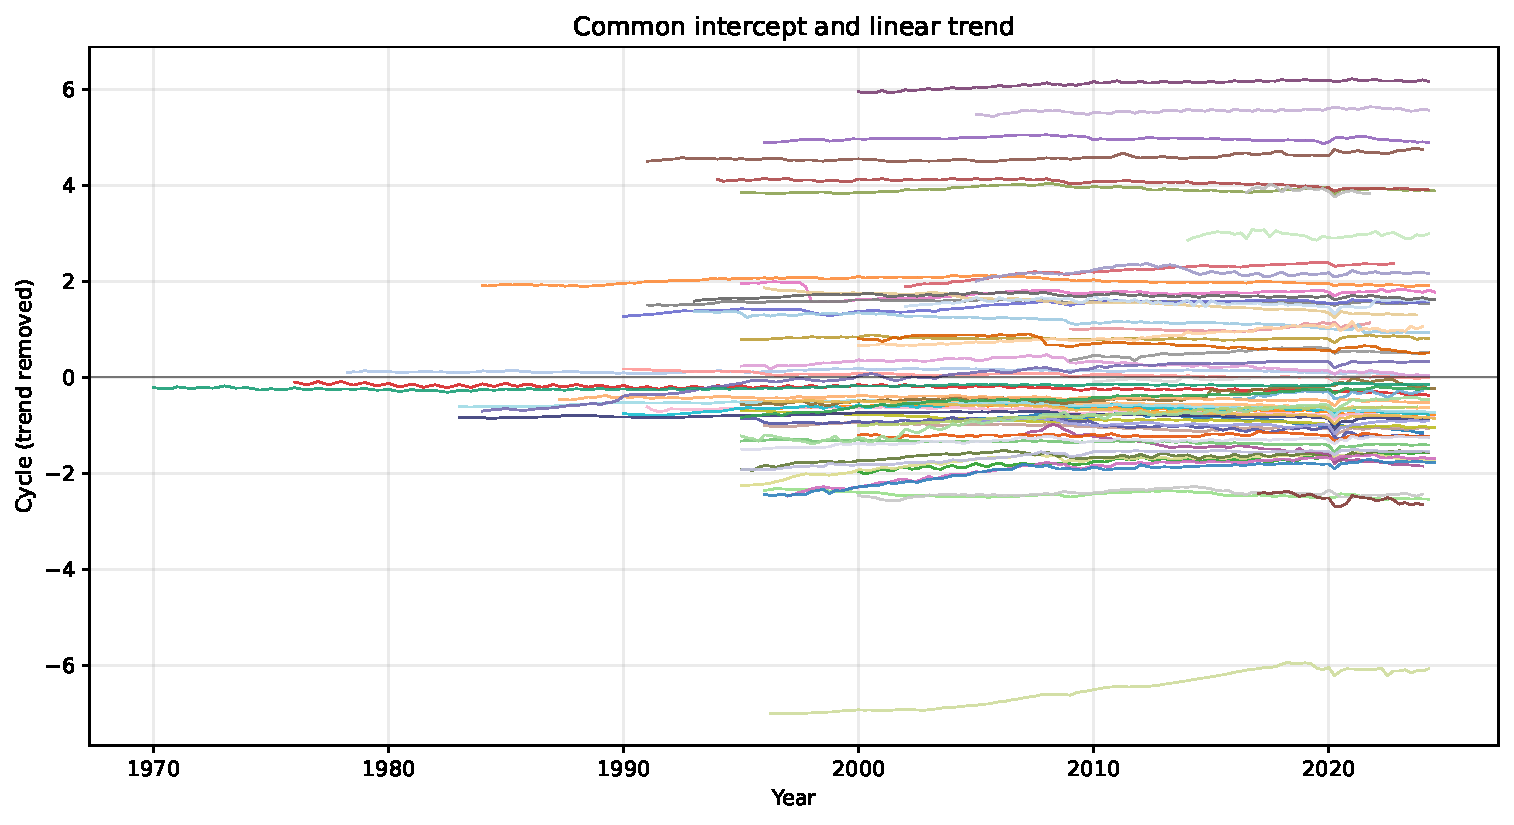
\includegraphics[width=0.75\textwidth]{figs/cycle_lin1970_common_ag.pdf}
\caption{Country cycles after removing the linear trend.}
\end{figure}
\clearpage
\section{Country-specific intercepts, common linear trend}
SOE sample from 1970Q1: log real GDP per worker. 62 countries, 6924 observations, 1970-Q1--2024-Q3. Fitted countries: 62. Observations: 6924. Log-likelihood: 17887.41.
Country intercepts $a_i$: mean -3.626, min -10.068, max 2.467. Common slope $g=0.0127$.
\begin{table}[h]
\centering
\caption{Regime AR(1) and transition matrix. Columns are regimes.}
\begin{tabular}{lccc}
\toprule
 & (0) & (1) & (2) \\
\midrule
$\mu$ & -0.2670 & 0.0000 & 0.2165 \\
 &  & --- &  \\ \addlinespace
$\sigma$ & 0.0224 & 0.0645 & 0.0097 \\
 &  &  &  \\ \addlinespace
$\rho$ & 0.9911 & 0.9166 & 0.9943 \\
 &  &  &  \\ \addlinespace
$\Pi_{0\cdot}$ & 0.9441 & 0.0240 & 0.0319 \\
 &  &  &  \\ \addlinespace
$\Pi_{1\cdot}$ & 0.0907 & 0.8039 & 0.1054 \\
 &  &  &  \\ \addlinespace
$\Pi_{2\cdot}$ & 0.0256 & 0.0129 & 0.9615 \\
 &  &  &  \\ \addlinespace
\bottomrule
\end{tabular}
\end{table}
\begin{figure}[h]
\centering
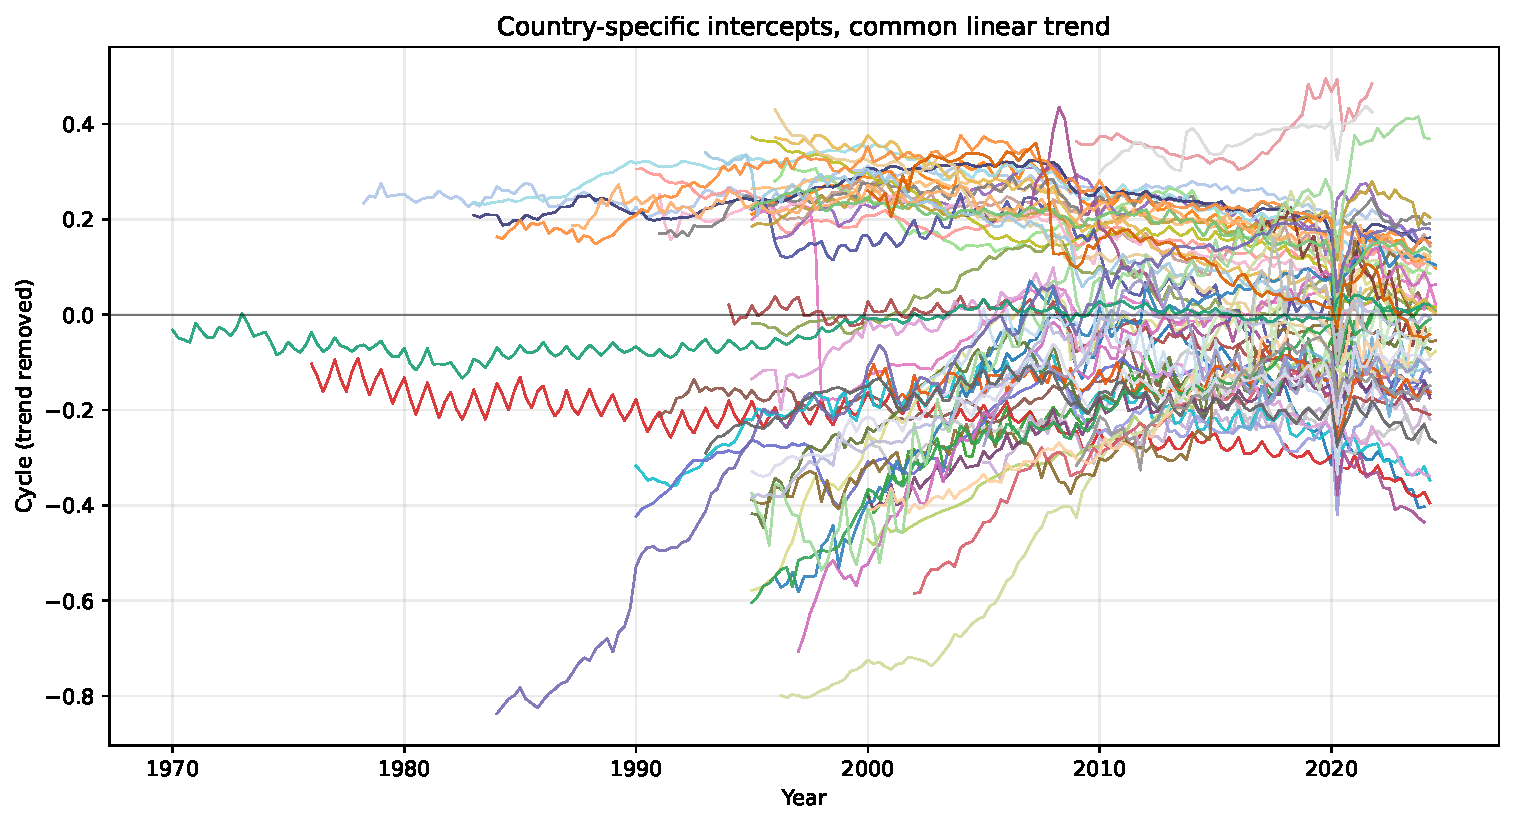
\includegraphics[width=0.75\textwidth]{figs/cycle_lin1970_ai_common_g.pdf}
\caption{Country cycles after removing the linear trend.}
\end{figure}
\end{document}
